\documentclass[a4paper, 11pt, english, fleqn]{article}
\usepackage[utf8]{inputenc}
\usepackage{babel}
%\usepackage{ngerman}
\usepackage{coordsys,logsys,color}
\usepackage{fancyhdr}
\usepackage{hyperref}
\usepackage{texdraw}				
\usepackage[T1]{fontenc}					
\usepackage{amsmath,amsfonts,amssymb}	
\usepackage[normalem]{ulem}	
\usepackage{listings}
\usepackage{graphicx}

\hypersetup{colorlinks=true, breaklinks=true, linkcolor=darkblue, menucolor=black, urlcolor=darkblue, citecolor=darkblue}

\pagestyle{fancy}

\renewcommand{\familydefault}{cmss}

\definecolor{fgcgray}{rgb}{0.4, 0.4, 0.4}
\definecolor{darkblue}{rgb}{0,0, 0.4}
\newcommand{\titlefont}[1]{\textcolor{black}{\fontseries{bx}\fontshape{n}\fontsize{30}{0pt} \selectfont #1}}
\newcommand{\titlepagef}[1]{\textcolor{black}{\fontseries{bx}\fontshape{n}\fontsize{14}{0pt} \selectfont #1}}

\newcommand{\gloss}[1]{\textcolor{glossb}{\fontsize{11}{0pt}\selectfont #1}}



\addtolength{\oddsidemargin}{-1.0cm}
\addtolength{\evensidemargin}{-1.0cm}
\addtolength{\headwidth}{2.0cm}
\addtolength{\textwidth}{2.0cm}

\setlength{\parindent}{0cm}

\renewcommand{\labelitemi}{$\circ$}
\renewcommand{\labelitemii}{$\diamond$}

\newcommand{\spaceline}[1][8pt]{\vskip #1}
\newcommand{\attrname}[1]{\textcolor{fgcgray}{\scriptsize #1}}

\newcommand{\comment}[1]{\spaceline[5pt] \textcolor{fgcgray}{\scriptsize #1} \spaceline[15pt]}

\makeatletter

\newcommand*{\project}[1]{\gdef\@project{#1}}


\def\@maketitle{
  %\begin{titlepage}
   
  \begin{center}
      \titlepagef{Softwareprojekt 2017}
      \spaceline
  \end{center}
  
  \begin{center}
      \parbox{\textwidth}{
        \spaceline
        \centering{\titlefont{Grobentwurf:\\ Realtime Mesh Utilities}}
        \par
        \spaceline
      }
  \end{center}
  
  \begin{center}
  \begin{tabbing}
  Petros Simiday \qquad \=
  Blerta Hamzallari \qquad \=
  Felix Griesau \qquad \=
  Marco Klamke \\
  Julius Lerm
  \>Lars Debor
  \>Sugandha Sachdeva  
  \>Simon Heinke
  \end{tabbing}
  \end{center}
 
  
  \spaceline[3em] {
    \begin{flushright}
    \begin{tabular}[t]{rl}
      \attrname{letzte Änderung:} & \@date
    \end{tabular}
    \end{flushright}
    \par
  }
  \spaceline[5.5em]
  %\end{titlepage}
}

\begin{document}
	
\lhead{\sc{Grobentwurf RMU}}	
\title{Grobentwurf: RMU}
\vspace{3 in}
\maketitle
\clearpage

\tableofcontents

\clearpage
\section{Basic structure of MNE-CPP}

MNE-CPP is a framework of tools and programs to analyze and work with MEG/EEG data.
mehr hinschreiben 

\begin{description}
	\item[deine muddi]

\end{description}

\clearpage

\section{Integration of the product into MNE-CPP}

The realtime mesh utilities are to be integrated into the structure of the MNE-CPP framework. Too provide a versatile interface, the utilities are organized inside a package within the library layer (see Figure 1).

\begin{center}
	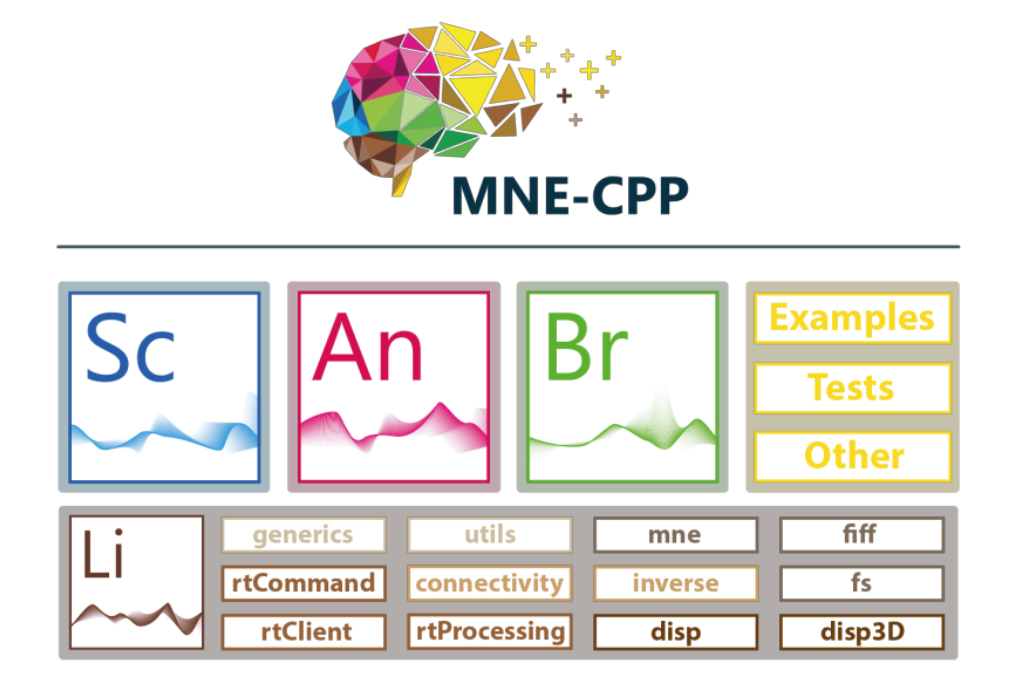
\includegraphics[width=10cm]{mne_architecture.png}
	\\
	{Figure 1 - Overview of the MNE-CPP basic architectural layout, including application and library layer.}
\end{center}

{pls insert klassendiagramm}

Later on, the features are to be ported to MNE-Scan (see section 1).

\section{Subdivision of program features}

\begin{description}
	
	\item[SCDC] 
	The surface constrained distance calculation algorithm receives a mesh data set as its input, which is stored inside a file. It then calculates approximate distances between vertices. When no further input arguments are provided, the SCDC algorithm calculates a full distance table, that is the distance between any vertex to any other vertex.
	When it receives a subset of the vertices as an additional argument, it only calculates the distances from said subset to every other vertex of the mesh. The SCDC algorithm stores its results inside a two-dimensional matrix.
	
	\item[Projecting]
	The projecting algorithm maps MEG/EEG-sensors to vertices of the mesh. In case of MEG-sensors, the orientation is known and thus a radial projection is applied in order to assign each sensor to a vertex. In case of EEG-sensors, the orientation is not know and a nearest-neighbor algorithm is used.
	The projecting algorithm then outputs the results of the calculation as an array of indices, which point to the respective vertices of the mesh.
	
	\item[Interpolation]
	The interpolation algorithm uses the results of both the projecting algorithm and the SCDC algorithm.
	Based on the distance table, it calculates a weight matrix for the later live interpolation. 
	Thus the interpolation algorithm receives three different inputs: the distance table created by SCDC, the sensors mapping and the actual sensor input, i.e. brain activity recorded by sensors over a period of time.
	The recorded brain activity gets passed to the interpolation algorithm either from an ongoing MME/EEG-Scan or a prerecorded data set, i.e. a file. 
	
	\item[Disp3D]
	In order to provide control over aspects of the interpolation within the MNE-CPP framework, a new function is added to the Disp3D tree model.
		
\end{description}

By dividing the realtime mesh utilities into the mentioned components, internal changes and extensions are easy to implement. Added to that, the single components can be reused elsewhere within the MNE-CPP framework.
\\

{pls insert sequenzdiagramm}

\clearpage
  
\end{document}
